

\tikzset{every picture/.style={line width=0.75pt}} %set default line width to 0.75pt        

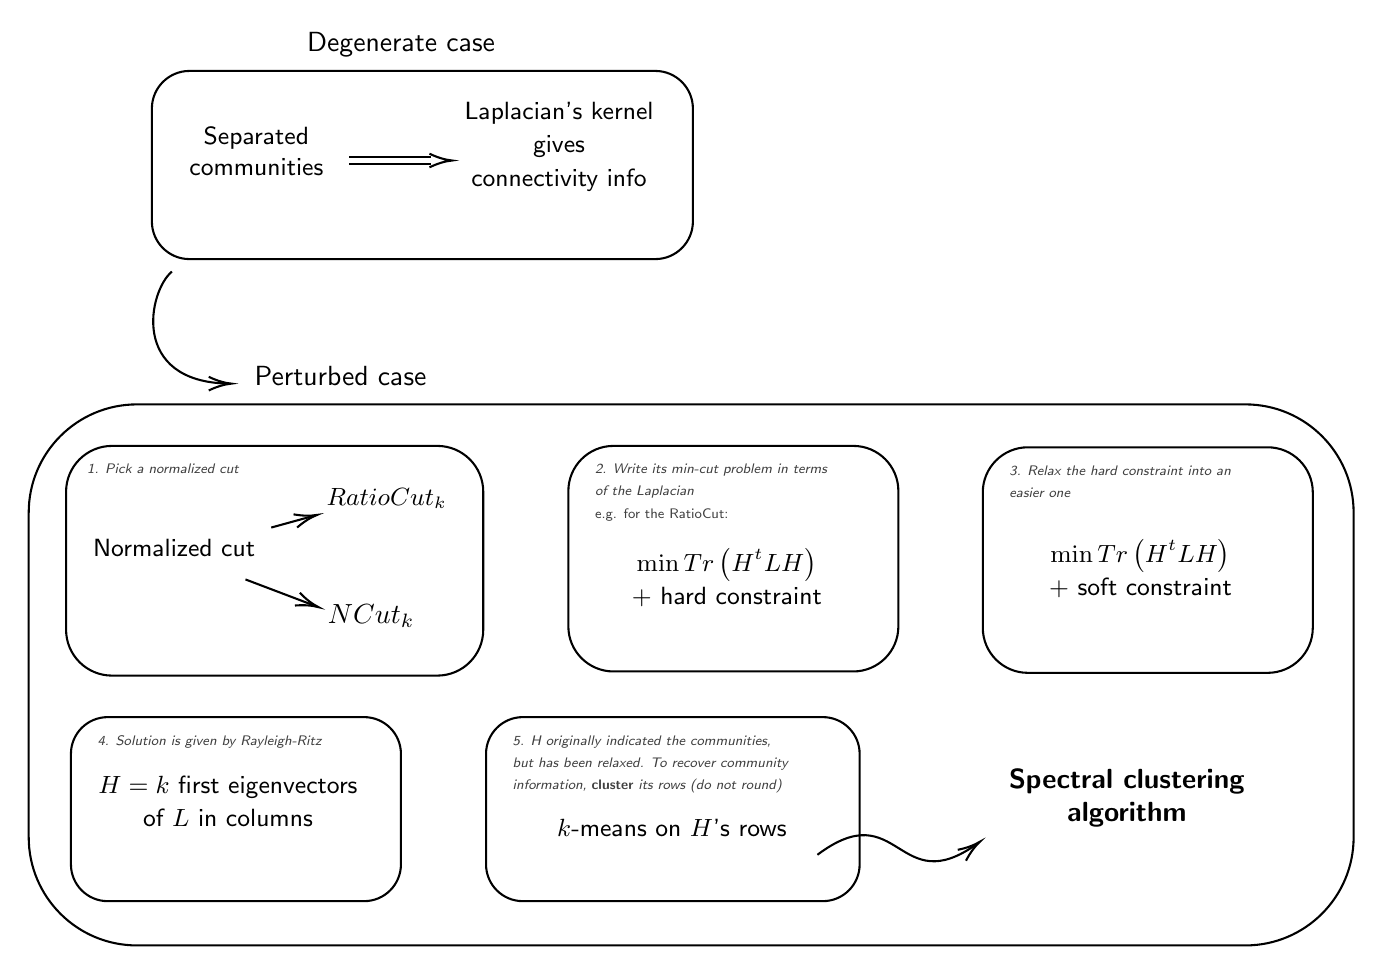
\begin{tikzpicture}[x=0.75pt,y=0.75pt,yscale=-1,xscale=1]
%uncomment if require: \path (0,515); %set diagram left start at 0, and has height of 515

%Rounded Rect [id:dp4742559449837811] 
\draw   (70.67,47.8) .. controls (70.67,37.79) and (78.79,29.67) .. (88.8,29.67) -- (313.2,29.67) .. controls (323.21,29.67) and (331.33,37.79) .. (331.33,47.8) -- (331.33,102.2) .. controls (331.33,112.21) and (323.21,120.33) .. (313.2,120.33) -- (88.8,120.33) .. controls (78.79,120.33) and (70.67,112.21) .. (70.67,102.2) -- cycle ;
%Rounded Rect [id:dp36300953291679927] 
\draw   (29.33,232.47) .. controls (29.33,220.24) and (39.24,210.33) .. (51.47,210.33) -- (208.2,210.33) .. controls (220.42,210.33) and (230.33,220.24) .. (230.33,232.47) -- (230.33,298.87) .. controls (230.33,311.09) and (220.42,321) .. (208.2,321) -- (51.47,321) .. controls (39.24,321) and (29.33,311.09) .. (29.33,298.87) -- cycle ;
%Rounded Rect [id:dp510487078419304] 
\draw   (271.33,232.07) .. controls (271.33,220.06) and (281.06,210.33) .. (293.07,210.33) -- (408.6,210.33) .. controls (420.6,210.33) and (430.33,220.06) .. (430.33,232.07) -- (430.33,297.27) .. controls (430.33,309.27) and (420.6,319) .. (408.6,319) -- (293.07,319) .. controls (281.06,319) and (271.33,309.27) .. (271.33,297.27) -- cycle ;
%Rounded Rect [id:dp7008246249036946] 
\draw   (471,232.73) .. controls (471,220.73) and (480.73,211) .. (492.73,211) -- (608.27,211) .. controls (620.27,211) and (630,220.73) .. (630,232.73) -- (630,297.93) .. controls (630,309.94) and (620.27,319.67) .. (608.27,319.67) -- (492.73,319.67) .. controls (480.73,319.67) and (471,309.94) .. (471,297.93) -- cycle ;
%Rounded Rect [id:dp7414306375759221] 
\draw   (11.33,242.47) .. controls (11.33,213.67) and (34.67,190.33) .. (63.47,190.33) -- (597.53,190.33) .. controls (626.33,190.33) and (649.67,213.67) .. (649.67,242.47) -- (649.67,398.87) .. controls (649.67,427.66) and (626.33,451) .. (597.53,451) -- (63.47,451) .. controls (34.67,451) and (11.33,427.66) .. (11.33,398.87) -- cycle ;
%Curve Lines [id:da21998107636183906] 
\draw    (80.33,126.33) .. controls (69.11,135.57) and (59.85,179.44) .. (107.54,180.32) ;
\draw [shift={(109,180.33)}, rotate = 180] [color={rgb, 255:red, 0; green, 0; blue, 0 }  ][line width=0.75]    (10.93,-3.29) .. controls (6.95,-1.4) and (3.31,-0.3) .. (0,0) .. controls (3.31,0.3) and (6.95,1.4) .. (10.93,3.29)   ;
%Rounded Rect [id:dp37954933488143205] 
\draw   (31.67,358.73) .. controls (31.67,348.94) and (39.61,341) .. (49.4,341) -- (172.93,341) .. controls (182.73,341) and (190.67,348.94) .. (190.67,358.73) -- (190.67,411.93) .. controls (190.67,421.73) and (182.73,429.67) .. (172.93,429.67) -- (49.4,429.67) .. controls (39.61,429.67) and (31.67,421.73) .. (31.67,411.93) -- cycle ;
%Rounded Rect [id:dp8175652045771994] 
\draw   (231.67,358.73) .. controls (231.67,348.94) and (239.61,341) .. (249.4,341) -- (393.93,341) .. controls (403.73,341) and (411.67,348.94) .. (411.67,358.73) -- (411.67,411.93) .. controls (411.67,421.73) and (403.73,429.67) .. (393.93,429.67) -- (249.4,429.67) .. controls (239.61,429.67) and (231.67,421.73) .. (231.67,411.93) -- cycle ;
%Curve Lines [id:da26907963961904546] 
\draw    (391.33,407.33) .. controls (430.93,377.63) and (429.7,429.94) .. (468.48,401.88) ;
\draw [shift={(469.67,401)}, rotate = 143.13] [color={rgb, 255:red, 0; green, 0; blue, 0 }  ][line width=0.75]    (10.93,-3.29) .. controls (6.95,-1.4) and (3.31,-0.3) .. (0,0) .. controls (3.31,0.3) and (6.95,1.4) .. (10.93,3.29)   ;

% Text Node
%\draw    (82.67,51.33) -- (161.67,51.33) -- (161.67,94.33) -- (82.67,94.33) 
%-- cycle  ;
\draw (85.67,55.33) node [anchor=north west][inner sep=0.75pt]  
[font=\small] 
[align=left] {\begin{minipage}[lt]{50.76pt}\setlength\topsep{0pt}
\begin{center}
{\fontfamily{cmss}\selectfont Separated}\\{\fontfamily{cmss}\selectfont 
communities}
\end{center}

\end{minipage}};
% Text Node
%\draw    (215.33,39.33) -- (323.33,39.33) -- (323.33,106.33) -- 
%(215.33,106.33) -- cycle  ;
\draw (218.33,43.33) node [anchor=north west][inner sep=0.75pt]   [align=left] {\begin{minipage}[lt]{70.49pt}\setlength\topsep{0pt}
\begin{center}
{\fontfamily{cmss}\selectfont {\small Laplacian's kernel gives
}}\\{\fontfamily{cmss}\selectfont {\small connectivity info}}
\end{center}

\end{minipage}};
% Text Node
\draw (144,9.33) node [anchor=north west][inner sep=0.75pt]   [align=left] 
{{\fontfamily{cmss}\selectfont Degenerate case}};
% Text Node
\draw (38,217.33) node [anchor=north west][inner sep=0.75pt]  
[font=\scriptsize] [align=left] {{\fontfamily{cmss}\selectfont 
\textit{{\tiny \color{gray!50!black} 1. Pick a normalized cut}}}};
% Text Node
%\draw    (36.33,249.67) -- (129.33,249.67) -- (129.33,274.67) -- 
%(36.33,274.67) -- cycle  ;
\draw (39.33,253.67) node [anchor=north west][inner sep=0.75pt]   [align=left] {\begin{minipage}[lt]{60.79pt}\setlength\topsep{0pt}
\begin{center}
{\fontfamily{cmss}\selectfont {\small Normalized cut}}
\end{center}

\end{minipage}};
% Text Node
%\draw    (150.33,220.33) -- (217.33,220.33) -- (217.33,248.33) -- 
%(150.33,248.33) -- cycle  ;
\draw (153.33,229.33) node [anchor=north west][inner sep=0.75pt]  
[font=\small] [align=left] {$\displaystyle \text{RatioCut}_{k}$};
% Text Node
%\draw    (151,281.33) -- (200,281.33) -- (200,313.33) -- (151,313.33) -- 
%cycle  ;
\draw (154,285.33) node [anchor=north west][inner sep=0.75pt]   [align=left] {$\displaystyle \text{NCut}_{k}$};
% Text Node
\draw (282.67,217.67) node [anchor=north west][inner sep=0.75pt]  
[font=\scriptsize] [align=left] {{\tiny \color{gray!50!black}
\textit{{\fontfamily{cmss}\selectfont 2. Write its min-cut problem in 
terms}}}\\{\tiny \color{gray!50!black} \textit{{\fontfamily{cmss}\selectfont of 
the 
Laplacian}}}\\{\tiny \color{gray!50!black} {\fontfamily{cmss}\selectfont e.g. for 
the 
RatioCut:}}};
% Text Node
\draw (299,258.33) node [anchor=north west][inner sep=0.75pt]   [align=left] 
{\begin{minipage}[lt]{70.81pt}\setlength\topsep{0pt}
\begin{center}
{\small $\displaystyle \min\text{Tr}\left( H^{t} LH\right)$}\\{\small 
{\fontfamily{cmss}\selectfont + hard constraint}}
\end{center}

\end{minipage}};
% Text Node
\draw (482.33,218.33) node [anchor=north west][inner sep=0.75pt]  
[font=\scriptsize] [align=left] {{\tiny \color{gray!50!black}
\textit{{\fontfamily{cmss}\selectfont 3. Relax the hard constraint into an 
}}}\\{\tiny \color{gray!50!black} {\fontfamily{cmss}\selectfont \textit{easier 
one}}}};
% Text Node
\draw (500, 254) node [anchor=north west][inner sep=0.75pt]   [align=left] 
{\begin{minipage}[lt]{68.24pt}\setlength\topsep{0pt}
\begin{center}
{\small $\displaystyle \min\text{Tr}\left( H^{t} LH\right)$}\\{\small 
{\fontfamily{cmss}\selectfont + soft constraint}}
\end{center}

\end{minipage}};
% Text Node
\draw (118.67,170.33) node [anchor=north west][inner sep=0.75pt]   
[align=left] {{\fontfamily{cmss}\selectfont Perturbed case}};
% Text Node
\draw (43,348.33) node [anchor=north west][inner sep=0.75pt]  
[font=\scriptsize] [align=left] {{\tiny \color{gray!50!black}
\textit{{\fontfamily{cmss}\selectfont 4. Solution is given by Rayleigh-Ritz}}}};
% Text Node 378
\draw (42,368) node [anchor=north west][inner sep=0.75pt]   [align=left] 
{\begin{minipage}[lt]{95.72pt}\setlength\topsep{0pt}
\begin{center}
{\small $\displaystyle H=k$ {\fontfamily{cmss}\selectfont first 
eigenvectors}}\\{\small {\fontfamily{cmss}\selectfont of }$\displaystyle L$ 
{\fontfamily{cmss}\selectfont in columns}}\\
\end{center}

\end{minipage}};
% Text Node
\draw (243,348.33) node [anchor=north west][inner sep=0.75pt]  
[font=\scriptsize] [align=left] {{\tiny \color{gray!50!black}
\textit{{\fontfamily{cmss}\selectfont 5. H originally indicated the 
communities,}}}\\{\tiny \color{gray!50!black} {\fontfamily{cmss}\selectfont 
\textit{but 
has 
been relaxed. To recover community}}}\\\textit{{\tiny \color{gray!50!black}
{\fontfamily{cmss}\selectfont information, \textbf{cluster} its rows (do not 
round)}}}};
% Text Node
\draw (263.33, 388.67) node [anchor=north west][inner sep=0.75pt]   
[align=left] {\begin{minipage}[lt]{84.6pt}\setlength\topsep{0pt}
\begin{center}
{\small $\displaystyle k${\fontfamily{cmss}\selectfont -means on 
}$\displaystyle H${\fontfamily{cmss}\selectfont 's rows}}
\end{center}

\end{minipage}};
% Text Node
\draw (479.33,364.67) node [anchor=north west][inner sep=0.75pt]   [align=left] {\begin{minipage}[lt]{89.49pt}\setlength\topsep{0pt}
\begin{center}
{\fontfamily{cmss}\selectfont \textbf{Spectral 
clustering}}\\{\fontfamily{cmss}\selectfont \textbf{algorithm}}
\end{center}

\end{minipage}};
% Connection
%\draw    (161.67,71.33) -- (207.33,71.33)(161.67,74.33) -- (207.33,74.33) ;
\draw    (165.67,71.33) -- (205.33,71.33)(165.67,74.33) -- (205.33,74.33) ;
\draw [shift={(215.33,72.83)}, rotate = 180] [color={rgb, 255:red, 0; green, 0; blue, 0 }  ][line width=0.75]    (10.93,-3.29) .. controls (6.95,-1.4) and (3.31,-0.3) .. (0,0) .. controls (3.31,0.3) and (6.95,1.4) .. (10.93,3.29)   ;
% Connection
\draw    (128.19,249.67) -- (148.41,244.1) ;
\draw [shift={(150.33,243.57)}, rotate = 164.59] [color={rgb, 255:red, 0; green, 0; blue, 0 }  ][line width=0.75]    (10.93,-3.29) .. controls (6.95,-1.4) and (3.31,-0.3) .. (0,0) .. controls (3.31,0.3) and (6.95,1.4) .. (10.93,3.29)   ;
% Connection
\draw    (115.77,274.67) -- (149.13,287.33) ;
\draw [shift={(151,288.04)}, rotate = 200.78] [color={rgb, 255:red, 0; green, 0; blue, 0 }  ][line width=0.75]    (10.93,-3.29) .. controls (6.95,-1.4) and (3.31,-0.3) .. (0,0) .. controls (3.31,0.3) and (6.95,1.4) .. (10.93,3.29)   ;

\end{tikzpicture}
